%File: formatting-instruction.tex
\documentclass[letterpaper]{article}
\usepackage{aaai}
\usepackage{times}
\usepackage{helvet}
\usepackage{courier}
\usepackage{graphicx}
\usepackage{xcolor}
\usepackage{natbib}
\usepackage{lmodern}
\usepackage[T1]{fontenc}
\bibliographystyle{aaai}
% Sudo Code packages
\usepackage[ruled, linesnumbered]{algorithm2e}

\usepackage{amsfonts}

\graphicspath{./..}

\frenchspacing
\setlength{\pdfpagewidth}{8.5in}
\setlength{\pdfpageheight}{11in}
\pdfinfo{
/Title (Reinforcement Learning: Parking lot)
/Author (Robert Horton)}
\setcounter{secnumdepth}{0}  
 \begin{document}

% The file aaai.sty is the style file for AAAI Press 
% proceedings, working notes, and technical reports.
%
\title{Networks \& Crowds:\\Spreading Bad Information Process  }
\author{Robert Horton\\
UCCS\\
1420 Austin Bluffs Pkwy,\\
Colorado Springs, Colorado 80918\\
}
\maketitle

% ----------------------------------------------- Abstract
\begin{abstract}
\begin{quote}
This paper briefy studies an instance of a graph given for the project whee the network is studied along with the influences that a node with a set amount of opinion and information can affect the whole network in different ways through connections to different original existent nodes.
\end{quote}
\end{abstract}

% ----------------------------------------------- Introduction
\section{Introduction}
In class, we discussed the Friedkin-Johnsen model of opinion dynamics, where opinions spread on a network but people always remember their initial opinions. To refresh our memory, the model works like this: We’re given a society with n individuals connected on a social influence network described by an $n \times n$ row-stochastic, directed, weighted adjacency matrix A. An edge $(i, \  j)$ (arrow pointing from i to j with weight aij means that node i gives a fraction aij of its attention to node j. Each node i has a susceptibility $\lambda i \in [0, \ 1]$, and we collect these susceptibilities into an $n \times n$ diagonal matrix $\Lambda = (\lambda_0, \ \lambda_1, \ . \ . \ . \ , \ \lambda_{n-1})_{diag}$. Given an initial vector of opinions $x(0) = (x_0(0), \ x_1(0), \ . \ . \ . \ , \ x_{n-1}(0))^T$ , the opinion at time $t$ is given recursively by
\begin{center}
	$x(t) = \Lambda \ A \ x(t - 1) + (I - \Lambda) \ x(0)$,\\ 
\end{center}
where $I$ is the $n \times n$ identity matrix. \\ \\
In this project, all questions consider the following weighted directed graph, with susceptibilities of $\lambda = (0.1,\ 0.2,\ 0.3,\ 0.4, \ 0.5, \ 0.6, \ 0.7, \ 0.8,\ 0.9, \ 0.95)$.  

\begin{center}
	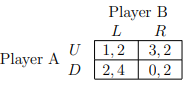
\includegraphics[scale=0.7]{./Images/Figure1.1} \\
	Figure 1.1
\end{center}
\begin{center}
	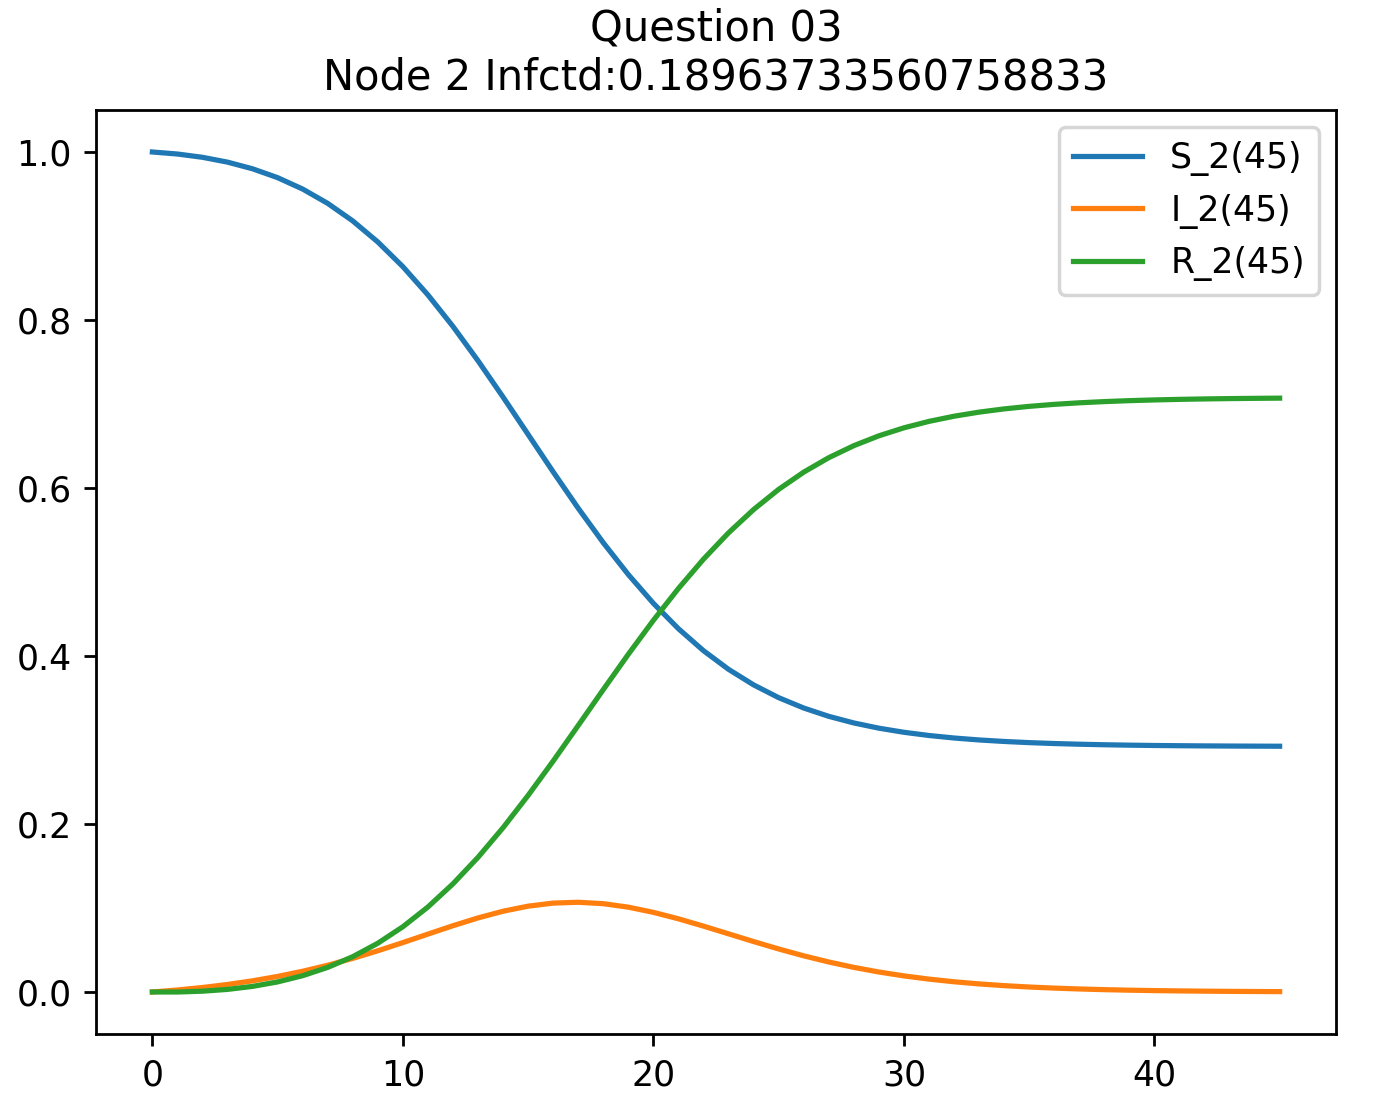
\includegraphics[scale=0.7]{./Images/Figure1.2} \\
	 Figure 1.2
\end{center}

\noindent Consider the following model of misinformation: let $x(0) = (0,\ 0, \ . \ . \ . \ , \ 0)^T$ so that everybody starts out at 0. Then, choose a node to influence (let’s say our influencing node $i$), and connect i to a new “fake” node whose initial “opinion” is 1. To make this connect, cut the weights of each of $i$’s out-edges in half, and give the new edge a weight of $0.5$. So the math works, the new fake node should have a single self-loop with weight $1$. See Figures 1.1 and 1.2 to show an example of a edge being added to node 9 to the new "fake node".  Because everybody starts out at 0, you can measure the effect of your misinformation simply by adding up everybody’s opinion. We’ll call this sum the propaganda value of your misinformation scheme, and denote it by $P(t) := \sum^{n-1}_{i=0} x_i(t)$ . An ineffective misinformation scheme would have $P(t)$ close to 0 for all time, but a very effective one would have $P(t)$ close to $n$.

% ----------------------------------------------- Implementation
\section{Implementation}  

Well to implement this first an object oriented approach was taken which was causing more over head and dependencies so a Jupyter Notebook was create to create the basic foundations for simpler to read and read code.  The following is a description of this implemented code.  First an adjacency matrix was built and hard codded into a python two dimensional array.  This we then proceed to use other code provided and earlier handout for the class to print the network out and to show that the network it represented correctly by the adjacency matrix.  
\begin{center}
	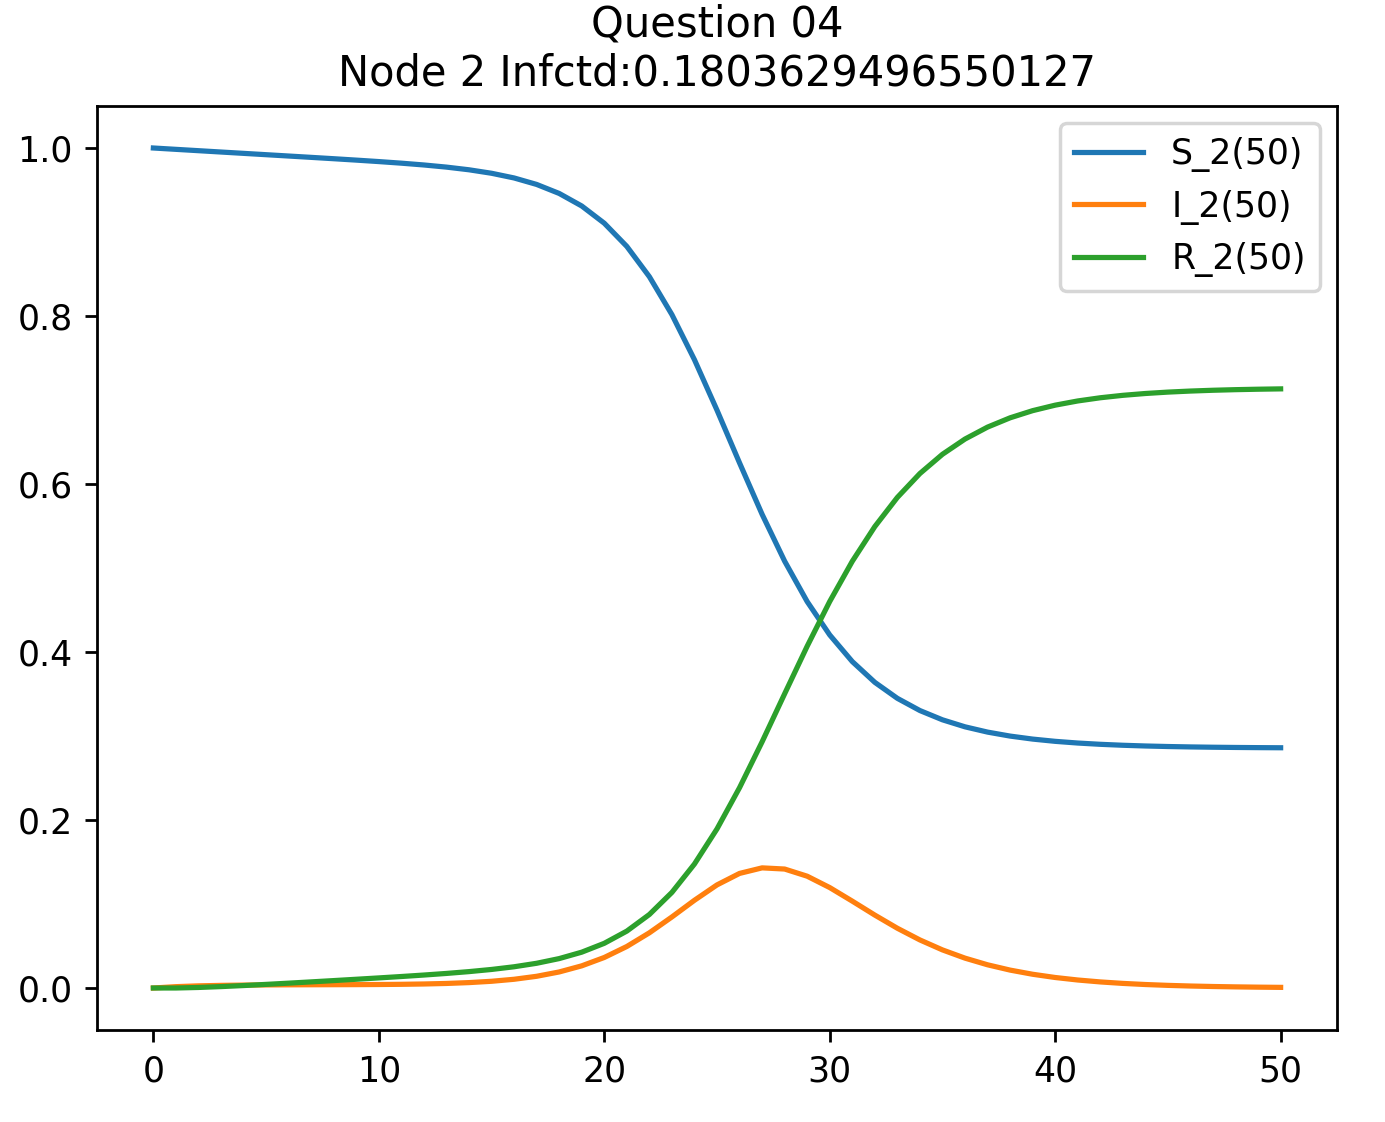
\includegraphics[scale=1.5]{./Images/Figure1.3} \\
	Figure 1.3
\end{center}
Although it might be hard to see the graph shown by Networkx that is used in a function provided to use, we can see that all the same nodes exist with the same existing edges as on the picture of the graph shown in Figure 1.1.  Now to demonstrate that we can add nodes to this adjacency matrix we build two more function that handle building the matrix and then will print it you to show that it works in connected a fake node to node 9 as in Figure 1.2.\\\\
The first function built I called addNodeToNetwork() which took two parameters which are the network we built an adjacency matrix for and the original opinion of all the existing nodes at time step $t=0$.  This functions take the network, as a two dimensional list and builds new rows with 0's added to the end of them and setting them to a new two dimension list to continue to modify before returning.  Next the two dimensional list will have a row of all zeros added at the bottom of the list. finally before returning the new network with an added node we set the new node to have a self loop and we also add a new opinion to the list or original opinions to represent the opinion of the new node which we will call the "fake node".  Both the list of opinion and new network are passed back. \\\\
Then the addBadEdgeToNetwork() method was created to be called right after adding a new node.  This function simply accepts three parameters to adjust the original network to having a edge between the fake node and what ever node is based as the 'node' argument.  To do this, the function multiplies every existing edge by 0.5 and then sets each element do that amount specific to the column in that node's row of edges.  Then a new edge of 0.5 is added between the fake node and the specified node.  This newly adjust network is then passed back.\\\\
After using the draw\_from\_matrix() function provided to us we can show that the matrix does in fact add a new edge.  We also checked the matrix was right by checking the console output of printing the matrix. \\
\begin{center}
	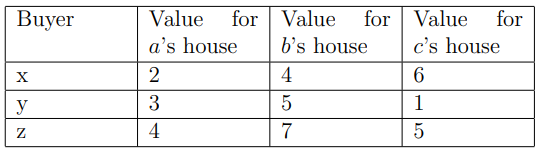
\includegraphics[scale=0.6]{./Images/Figure1.4} \\
	Figure 1.4
\end{center}
As we can see a new node has been added and the only added edge are the self loop to itslef and the new edge between node 9 and node 10, the fake node.\\\\
After verifying that this was working we used the friedkin\_johnsen() provided to us through class handouts and modified it to print out a little bit more verbose information when setting its keyword argument, show\_plot, is set to true.  This function does what has already been discussed in class by essentially using the equation as described in the introduction.  By preforming these different time steps of Friedkin-Johnsen model we were able to map the rate at which the information, or "opinion", of the "fake" spreads depending on the node that it is connected to. To perform each instance of when a different node could be connected to the "fake" node we make an abstract layer to call of the methods previously discussed so that this method or model can be called upon in a for loop of each possible neighbor that the fake node could have a connection from.  Within this model a fresh new network of the original network is made sure to be passed in to this model to represent the only connection between the fake node and any other pre-existing node.\\
Along with executing every possible connection, a list was made to capture the overall propaganda value of the network at each time step.  Another function was written to show this value as well as the opinion of each node at each iterated time step through the model and were used to display the results through other implemented methods plotAllProagandaValOverTime() \& plotAllProagandaValOverTime() to plot them individually between simulation runs and to call at the end of the for loop of all possible simulation runs to map all possible outcomes of $P(t)$ values specific to the node that the fake node was being connected from.  Unit test were also written to make sure that basic functionality is maintained through out the completion and development of this project.

% ----------------------- Execution 
\subsection{Execution}
To help mitigate any dependencies that may cause issues with running the program a requirments.txt file was provided which can be used with the below command to make sure that all the libraries used for this project are pre installed.\\
\begin{center}
py -m pip install -r requirments.txt\\
\quad \\
\end{center}
Execution is set up to simply run the missinformationProjecy.py file with the commad\\
\begin{center}
py project03.py\\
\quad \\
\end{center}
from the same working directory as this file. When running this file, without modifying it, it should display different graphs that will require the user to exit out of to continue to run the file.  If the user wishes to run the file without the printout of all the graphs they must go through and change the plot\_resultargument to False as well as comment out the method calls of the functions timestepsToPTable() and plotAllProagandaValOverTime().  This will still display the tables required of in the deliverables and will be presented as such to exclude ambiguity with which deliverables are what. 
Include in this zip are other unit tests and outputs they were saved from previous runs to make sure that the grader is getting all the required deliverables \\
% ----------------------- Analyisis 
\subsection{Analyisis}
After personal execution with collected data and observations, I was then able to continue with providing the deliverable for the project.  First off a quick overview of each overview asked of in the project and what it consists of.\\\\
\begin{enumerate}
	\item Implement the Friedkin-Johnsen model on the given graph. As always, I will check for copy-pasted code from the internet so if you use someone else’s code, you must cite them.
	\begin{enumerate}
		\setcounter{enumi}{1}
		\item  Deliverable 1: Either the computer code for your implementation, or a complete description of the maths you used to prove the other deliverables. CS 5740 students, this deliverable includes your epidemic code as well. 
	\end{enumerate}
	\item If you want to influence opinions over the short-term, which node should you influence?
	\begin{enumerate}
		\setcounter{enumi}{2}
		\item  Deliverable 2: The graph has 10 nodes; create a table which shows $P(1)$ (the total opinion of society after 1 time step) for each node to be influenced. That is, compute $P(1)$ in the case that you influence node 0; then compute $P(1)$ in the case that you influence node 1, and so on. If you care most about $P(1)$ (society’s opinions in the very short term), which node is best to influence? Which is worst? Write a few sentences explaining why you think this is the case.
	\end{enumerate}
	\item If you want to influence opinions over the long-term, which node should you influence?	
	\begin{enumerate}
		\setcounter{enumi}{3}
		\item Deliverable 3: The graph has 10 nodes; create a table which shows $P^\infty := \lim_{t to \infty} \ P(t)$ (the opinion that society converges to after a long time) for each node to be influenced. That is, compute $P^\infty$ in the case that you influence node 0; then compute $P^\infty$ in the case that you influence node 1, and so on. If you care most about $P^\infty$ (society’s opinions in the very long term), which node is best to influence? Which is worst? Write a few sentences explaining why you think this is the case. If the answer is different from what you got in Deliverable 2, try to explain why.\\\\
	\end{enumerate}
\end{enumerate}

% ----------------------- Delveriable 1 
\subsection{ Deliverable 1 }
The code for this assignment will be turned in via a zip file, so this will take care of Deliverable 1

% ----------------------- Delveriable 2
\subsection{ Deliverable 2 }
For Deliverable 2 we are to evaluate the overall networks opinions in the short term.  After exciton of only 10 steps we can see a fairly quick convergence in the different nodes and the opinions in the network over just that many time steps.  What we are interested in is which connection from one of the existing node to the fake node will cause the networks propaganda value to get closer to 0, meaning that this fake nodes new connection to it is highly ineffective.  The closer the propaganda value gets to $n$, the size of the network minus the fake node, the more effective the propaganda is from the fake node. So when looking at the graph in Figure 1.5 we see all the propaganda values of the network when the fake node has an edge coming to it from one of the 10 (0-9) existing nodes.
\begin{center}
	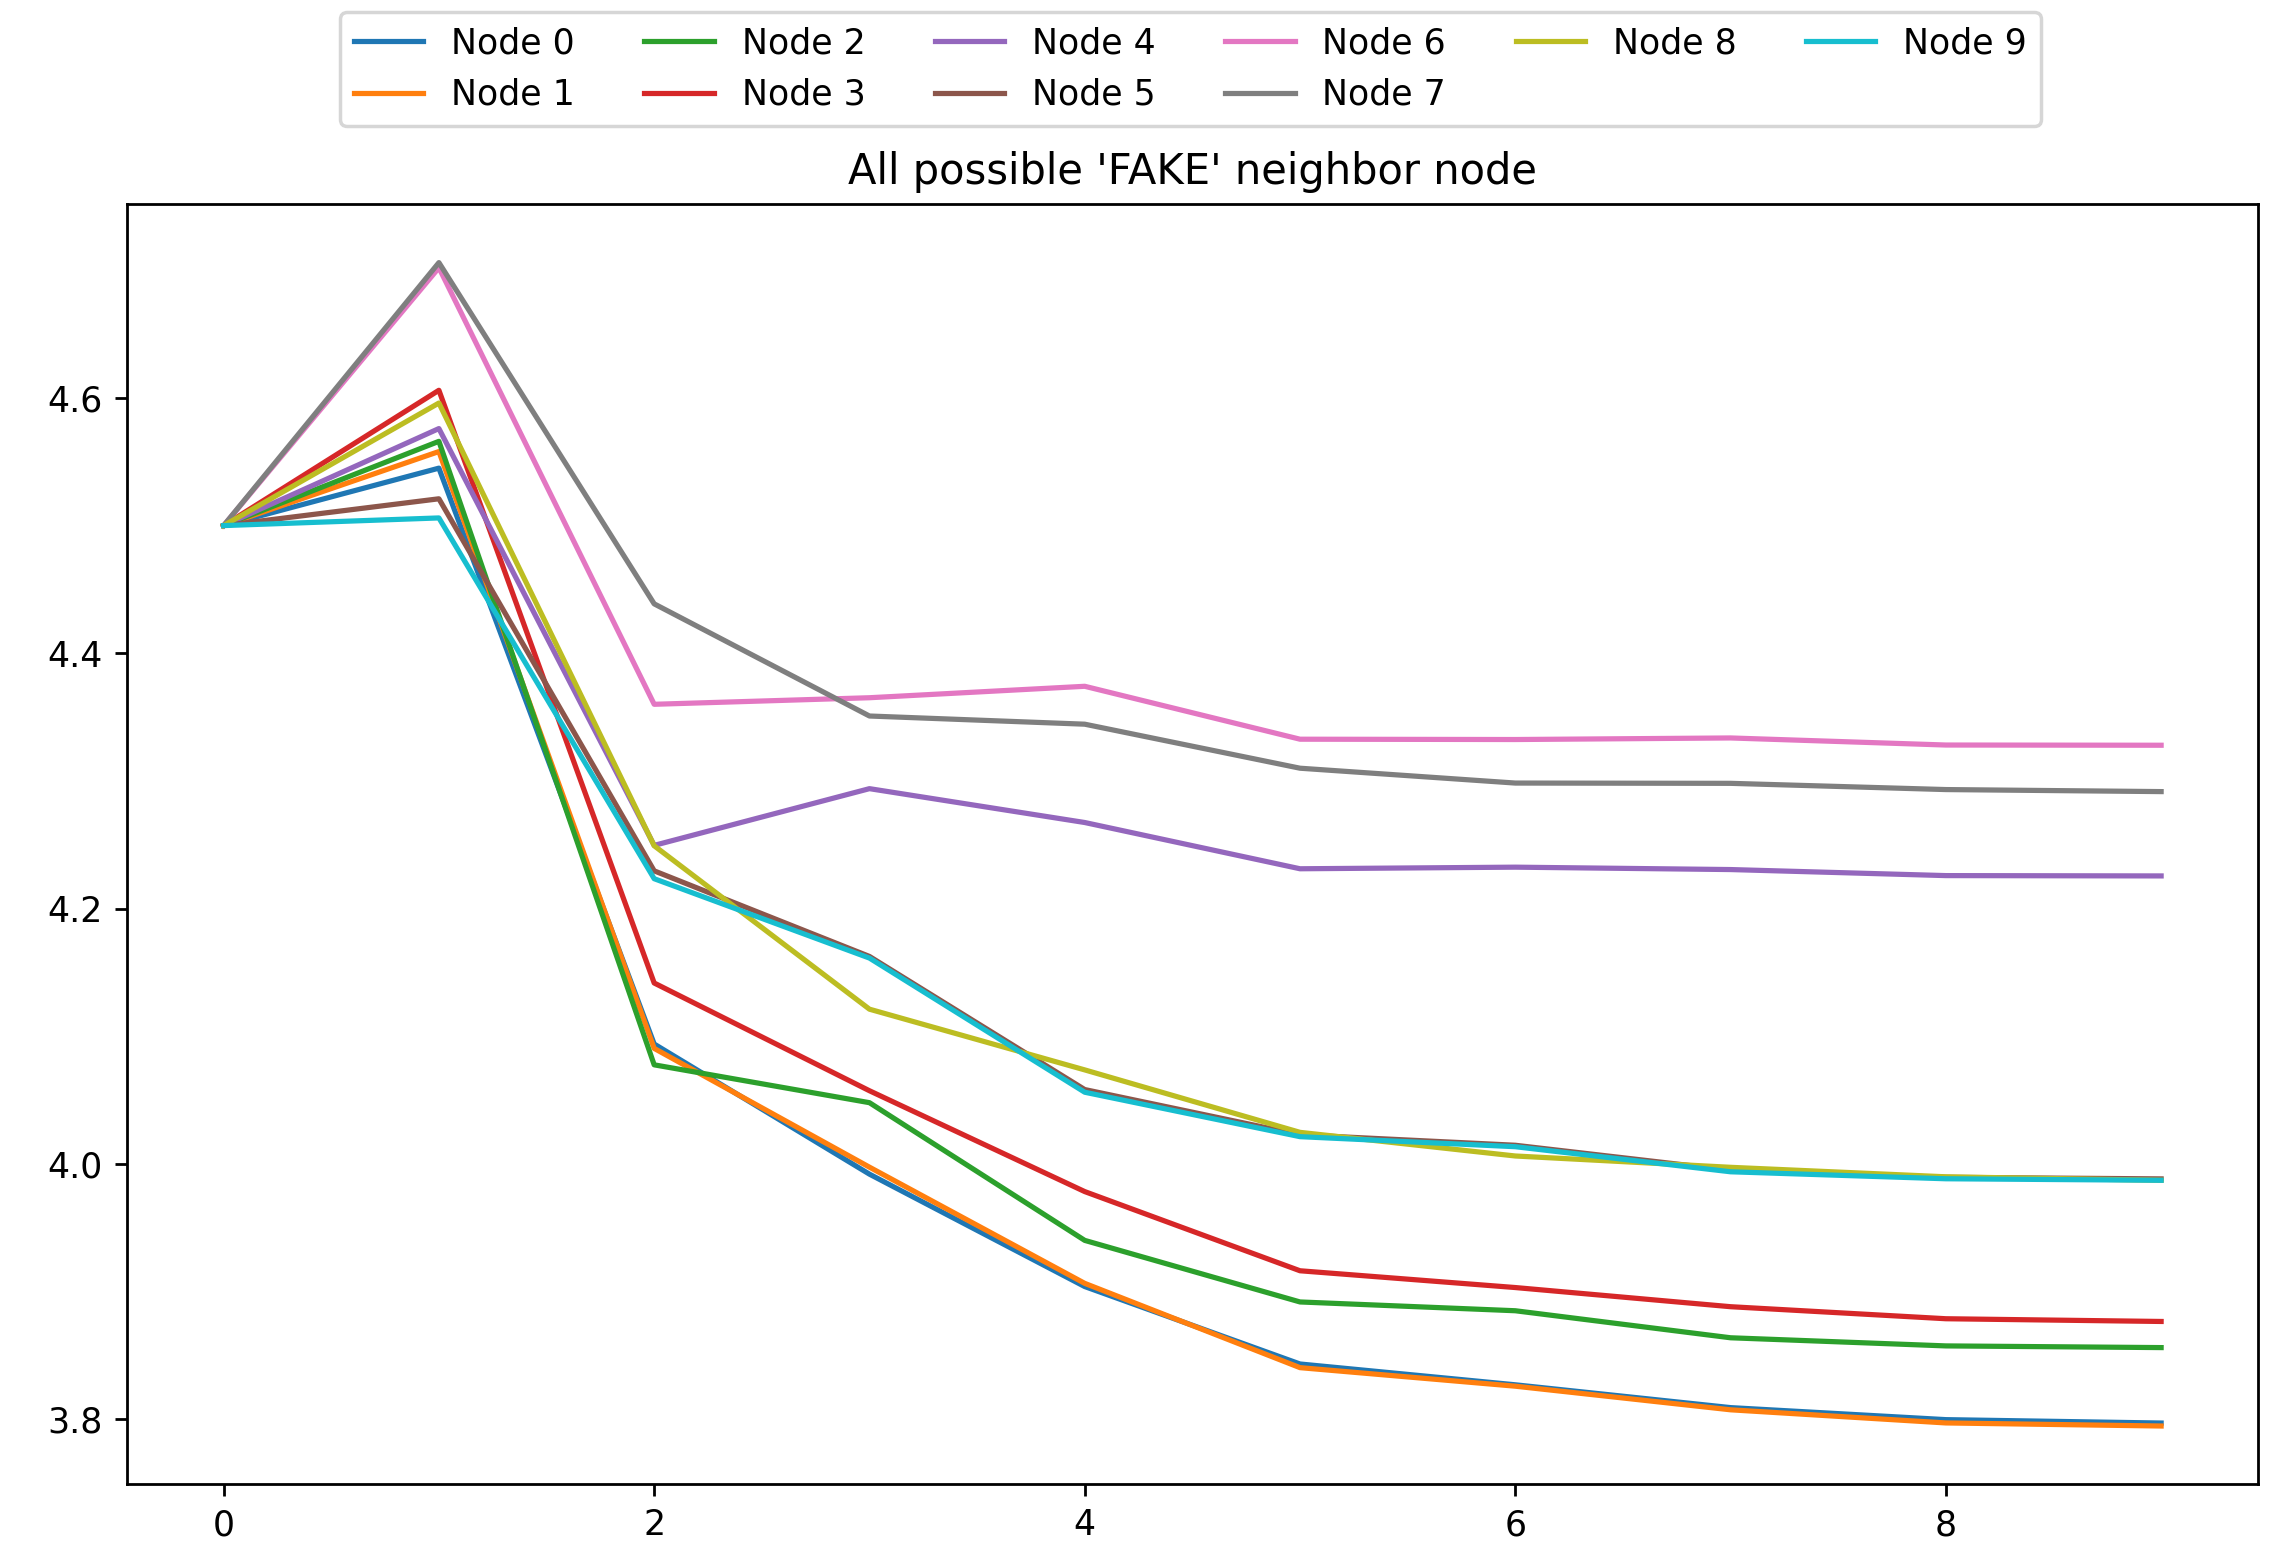
\includegraphics[scale=0.34]{./Images/Figure1.5} \\
	Figure 1.5
\end{center}
As we can see from this chart in Figure 1.5, nodes 9 and 5 seem to have the lowest propaganda values after the first initial time step.  The chart seems to show a slightly sharp up tick in p values among the networks for the different connections made between the original network and the fake node.  We can see that nodes 6 and 7 seem to have the highest p value when connected to the fake connection.  We can see that the p-value jumps up to 4.7.  When looking at the graph in figure 1.2, it seems to make since as the first to set of nodes that seem to go the same high point being also the lowest in the network of just above 4.5.  This makes since because these nodes share most of the connection of other incoming edges that have not yet been affected by the p-value.  Since they have a lot more edge coming from original value it is smaller.  As for nodes 6 and 7 we see that these two nodes are some of the few that node 4 listens to while having many listen to it.  For this reason when connected to these few nodes that are directly connected to node 4 seem to have a more rapid expansion of p-values after the first time step.  

% ----------------------- Delveriable 3
\subsection{ Deliverable 3}
For Deliverable 3 we are to evaluate the overall networks opinions in the long term. Although it seems to converge rather quickly and only 10 iterations is really needed, 99 iterations were perfromed foe each possible node connection and below is a table that show these values 
\begin{center}
	\begin{tabular}{| c | c | c | c | c |}
		\hline  
		 $P(t)_{ij}= (node_i, \ node_j)$    & t=0 & t=1 & . . . & t=99\\
		\hline
		 (0, fake) & 4.5 & 4.545  &  . . .  &  3.78796\\  
		\hline
		 (1, fake) & 4.5 & 4.558 & . . .  & 3.85022 \\ 
		\hline
		(2, fake) & 4.5 & 4.566  & . . .  & 3.87118 \\  
		\hline
		(3, fake) & 4.5 & 4.606  & . . .  & 3.87118 \\  
		\hline
		(4, fake) & 4.5 & 4.576  & . . .  & 4.22463 \\  
		\hline
		(5, fake) & 4.5 & 4.521  & . . .  & 3.98291 \\   
		\hline
		(6, fake) & 4.5 & 4.702  & . . .  & 4.32722  \\  
		\hline
		(7, fake) & 4.5 & 4.706  & . . .  & 4.29062  \\  
		\hline
		(8, fake) & 4.5 & 4.596  & . . .  & 3.98346  \\  
		\hline
		(9, fake) & 4.5 & 4.506  & . . .  &  3.98179 \\  
		\hline
	\end{tabular}
\end{center}
After looking at the table we see that node 1 seem to have the lowest p-value meaning it is the least effective node to connect to when trying to maximize the p-value to spread misinformation.  However, node 6 seems to be be the best connection for the fake node to have a connection to it from since it yields a higher p-value and is the most effective on the network. This makes since as we look at the graph provided in Figure 1.5 and see although the lower nodes, 9 and 5, only get as low as just above 0.4.  We see that nodes 0 and 1 seems to get to the lowest p-value over a long period time to almost as low as 3.8.  Although the initial effect on the network seems to have and seemingly average spike in p-value compared to the rest, it does drop to be the lowest p values over  a long period of time.  This can probably be attributed to the fact that these nodes do not seem have heavy influence on any of the highly influential nodes with lots of other nodes listening to them.  This explains why the p-values seem to have lasting affect but for nodes like 6, 7, and 4 with create networks with high p-values because  the nodes are or share strong connections with highly influential nodes that overall affect the whole network.   

% ----------------------------------------------- Conclusion
\section{Conclusion}

In conclusion we can see that for a complete graph with a given set of opinions has some very specific phenomenons that seem to happen. Through other generated table in the code written we wee also able to see that only nodes with high opinion values seem to vary greatly for their original opinions so ultimately nodes with lower opinions are going to ultimately come out of the simulations with an opinion that is not very different from its original.  Nodes like 9 for example, with a high opinion of 0.95 will drop down to as low as 3.7 as seen in Figure 1.6.
\begin{center}
	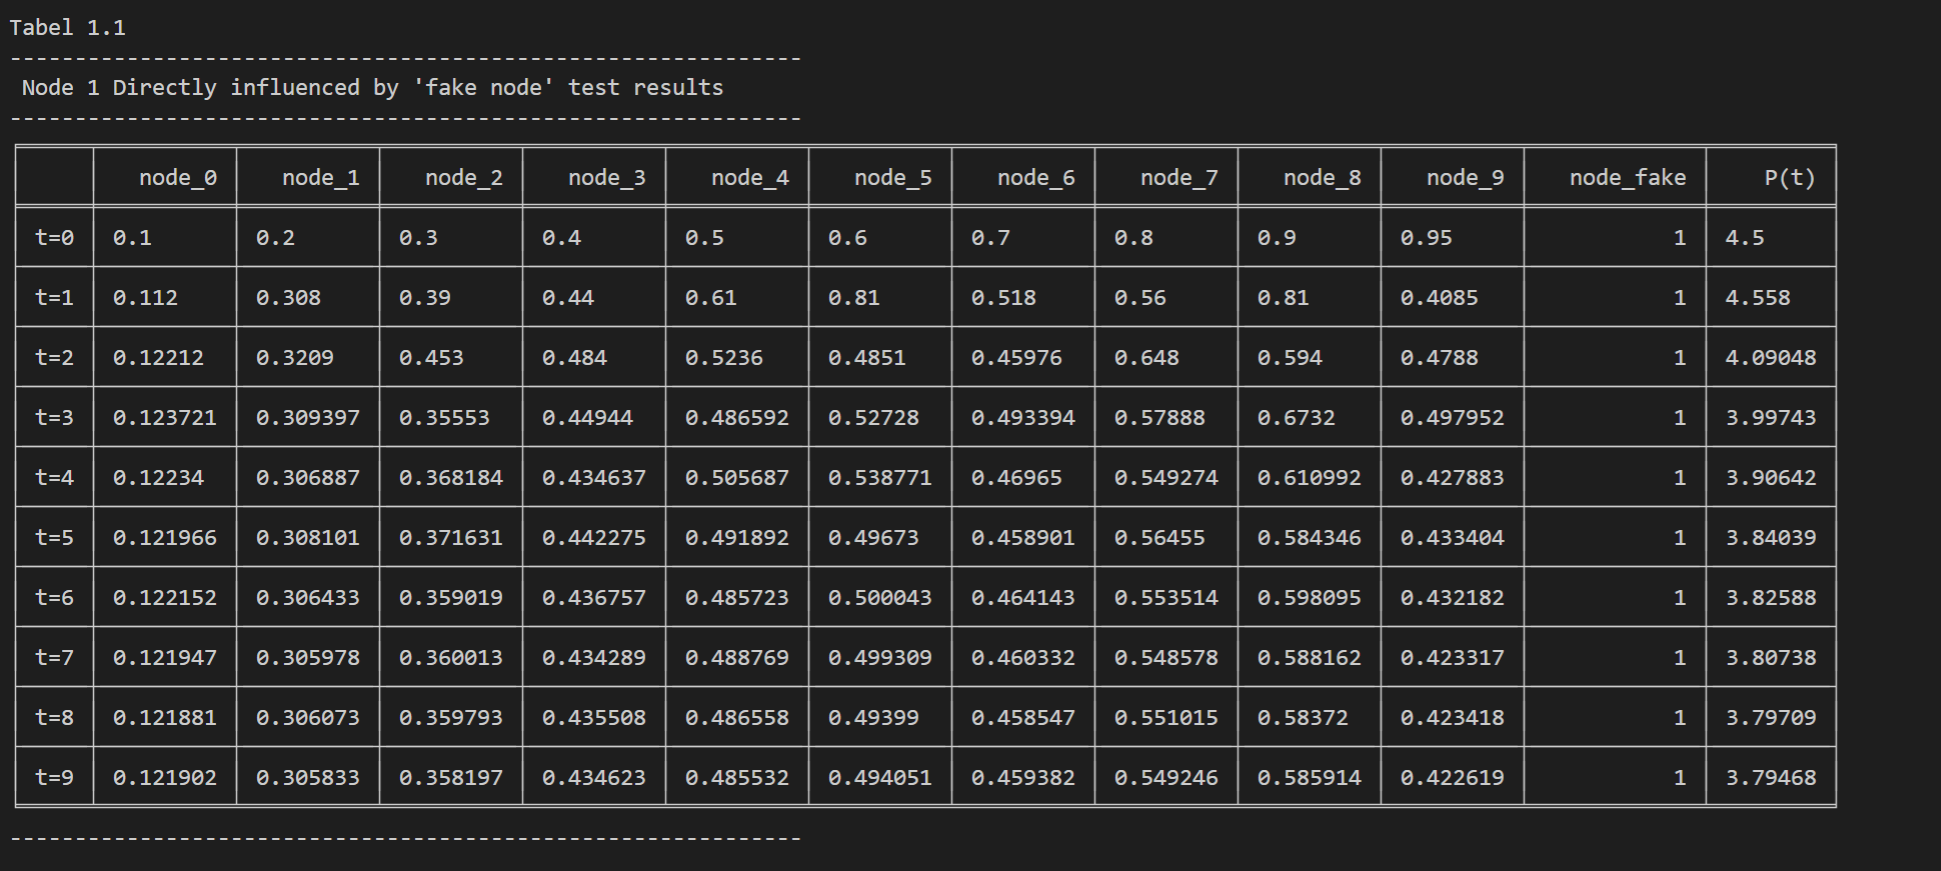
\includegraphics[scale=0.4]{./Images/Figure1.6} \\
	Figure 1.6
\end{center}
All these tables for all possible connections can be found in the provided text output.txt file turned in with the zip for this assignment.

% ----------------------------------------------- References 
\section{References}
Credit to Dr. Philliph Brown's Jupyter note books and other class handouts

\end{document}